
\section{Lecture 7 - 02.02.21}

\subsection{Projective algebraic sets}

We recall the definition of the projective space of a vector space $E$ from last time. 

\begin{definition}
Let $E$ be a $n+1$-dimensional vector space over a field $k$. The projective space of $E$, denoted $\P(E)$, is the set $(E\setminus \{0\})/\sim$, where $x\sim y \iff \exists \lambda \text{ such that } x=\lambda y$. 
\end{definition}

If $E=k^{n+1}$ then we denote $\P(E)$ by $\P^n(k)$, which we call projective $n$-space. We have a map 
\begin{align*}
    k^{n+1}&\longrightarrow \P^n(k) \\
    (x_0, \ldots, x_n)\longmapsto [x_0:\cdots :x_n]
\end{align*}
We call $(x_0, \ldots, x_n)$ the homogeneous coordinates. 

\begin{definition}
Let $E$ be a $n+1$-dimensional vector space over $k$, $0\leq m\leq n$ be an integer and $F$ a $m+1$-dimensional subspace of $E$. The image of $F\setminus \{0\}$ in $\P(E)$ is called the projective subspace of dimension $m$, denoted $\overline{F}$. 
\end{definition}

If $m=0$ then $\overline{F}$ is a point. If $m=1$ then $\overline{F}$ is a line. If $m=n-1$ then $\overline{F}$ is a hyperplane. 

\begin{proposition}
Let $E$ be a $n+1$-dimensional vector space over $k$.Let further $V, W$ be two projective subspaces of $\P(E)$ with dimension $r$ and $s$ respectively such that $r+s-n\geq 0$. Then $V\cap W$ is a projective subspace of dimension greater than $r+s-n$. In particular, $V\cap W\neq \emptyset$.  
\end{proposition}

\begin{remark}
     This proposition is not true in the affine case. This is due to the existance of paralell lines, which are both affine subspaces, but has empty intersection. 
\end{remark}

\begin{proof}
We write $V=\overline{F_V}$ and $W=\overline{F_W}$ for $F_V, F_W$ two subspaces of $E$ with dimension $r+1$ and $s+1$ respectively. Note that the intersection of two vector subspaces is again a vector subspace, hence $\overline{F_V\cap F_W}$ is actually a projective subspace. Moreover we have:
\begin{align*}
    dim(F_V\cap F_W) &= dim (F_V) + dim (F_W) - dim(F_V+F_W) \\
    &\geq (r+1)+(s+1)-(n+1) \\
    &= r+s-n+1
\end{align*}
This means that $dim(V\cap W) = dim(\overline{F_V}\cap \overline{F_W})=dim(\overline{F_V\cap F_W})\geq r+s-n$.
\end{proof}

\begin{example}
     Two distinct lines in $P^2(k)$ meet at a unique point. 
\end{example}



\subsection{Homography}

We will not cover this in detail, but we quickly mention what these are. 

\begin{definition}[Homography]
Let $u$ be a vector space isomorphism on a vector space $E$, i.e. $u\in GL(E)$. The induced map $\overline{u}:\P(E)\longrightarrow \P(E)$ is called a homography. These are isomorphisms of projective spaces, and are as you can see the ones induced by vector space isomorphisms. 
\end{definition}


\subsection{What does projective space look like?}

For easy visualization we let $k=\R$. Since we are on our goal to understand and prove Bezouts theorem, we are mostly interested in $\P^2(k)$, so lets try to visualize and understand $\P^2(\R)$. I did this a bit in \ref{lec5:visualization} but it never hurts to do it again. 

We start by drawing $\R^3$, as this is where we get our points from. 
\begin{center}
\def\svgwidth{0.4\textwidth}
\input{inkscape/3axes.pdf_tex}
\end{center}

As we have $x=y$ in $\P(E)$ whenever there exists a $\lambda$ such that $\lambda x = y$ we get in our coordinates that $[x:y:z] = [\frac{x}{z}:\frac{y}{z}:1]$ which means that we can just look a the plane $z=1$ in $\R^3$. 

Every point on that plane uniquely determines a line through the origin, as visualized below. 

\begin{center}
\def\svgwidth{0.4\textwidth}
\input{inkscape/projective_point.pdf_tex}
\end{center}

This means that much of $\P^2(\R)$ acts like $\R^2$, and we get the intuitive equality $\P^2(\R) ``='' \R^2 \cup \{ \text{points at infinity}\}$. Lets make this a bit more rigorous. 

We define $H=V(z)\subseteq \R^3$, and $\overline{H}\subset \P^2(\R)$ to be its projective space. We then set $U=\P^2(\R)\setminus \overline{H}$. There is a bijection 
\begin{align*}
    \phi: U&\longrightarrow \R^2 \\
    [x:y:z]&\longmapsto (\frac{x}{z}, \frac{y}{z}) \\
    [x:y:1]&\longmapsfrom (x, y)
\end{align*}

Furthermore, the inclusion $\overline{H}\hookrightarrow \P^2(\R), [x:y:0]\mapsto [x:y:0]$ splits by the map
\begin{align*}
    \P^2(\R)&\longrightarrow \overline{H} \\
    [x:y:z]&\longmapsto [x:y:z]
\end{align*}
meaning that we have $\P^2(\R)= \overline{H}\coprod U = \P^1(\R)\coprod \R^2$. These we think about as ``points at infinity'' and ``points at a finite distance'' respectively. 

\begin{problem}
     What does $\P^1(\R)$ look like?

\begin{solution}
By the same argument as earlier we can look at the $y=1$ line in $\R^2$ to determine how $\P^1(\R)$ looks. Every point on the line determines uniquely a line with a unique slope $m$. All possible slopes $m\in \R$ are hit by one such line, except $m=0$. This line never intersects the $y=1$ line, and is hence designated as the ``point at infinity''. As we have a line isomorphic to $\R$, with the same ``point at infinity'' in both ends, this shape is homeomorphic to the circle $S^1$. We think of this as folding the real line into a circle and gluing it together at this ``point at infinity''.
\end{solution}
\end{problem}

Another way to visualize projective space is to use spheres. Since the space $\R^3\setminus \{0\}$ is homeomorphic to $S^2$ we can study that instead. A line through the origin intersects the sphere at two points. These points are antipodal. We can then reduce to thinking about the half-sphere instead.

\begin{center}
\def\svgwidth{0.4\textwidth}
\input{inkscape/projective_2-space.pdf_tex}
\end{center}

We still have identified the antipodal points at the equator, but all other points correspond to a unique line, i.e. a point in projective space. The points on the equator are then the ``points at infinity'' while the non-equatorial points are the ``points at finite distance''. As with $\P^1(\R)$ we can think of this as gluing each line in the plane $z=1$ to its endpoints at infinity. 

\begin{example}
We can also study projective lines in $\P^2(\R)$. Lets see what happens with ``parallel lines'', as these are the ones we are trying to get rid of using projective space instead of affine. 

A $1$-dim projective line is the image of a $2$-dim subspace of $\R^3$, i.e. a plane. This means that the points at finite distance of the projective line is the intersection of that plane and the plane $z=1$. We draw this for two projective lines.

\begin{center}
\def\svgwidth{0.4\textwidth}
\input{inkscape/paralell_projective_lines.pdf_tex}
\end{center}


We see that the two planes cut out two ``parallel lines'' on the plane. But, the planes also intersect elsewhere, namely at the red line in the $xy$-plane. That line determines a point at infinity in $\P^2(\R)$, hence the two projective lines do indeed meet at a point. 

\end{example}

Another example is the affine algebraic set given by $C=V(XY-Z^2)\subseteq \R^3$. 
\begin{center}
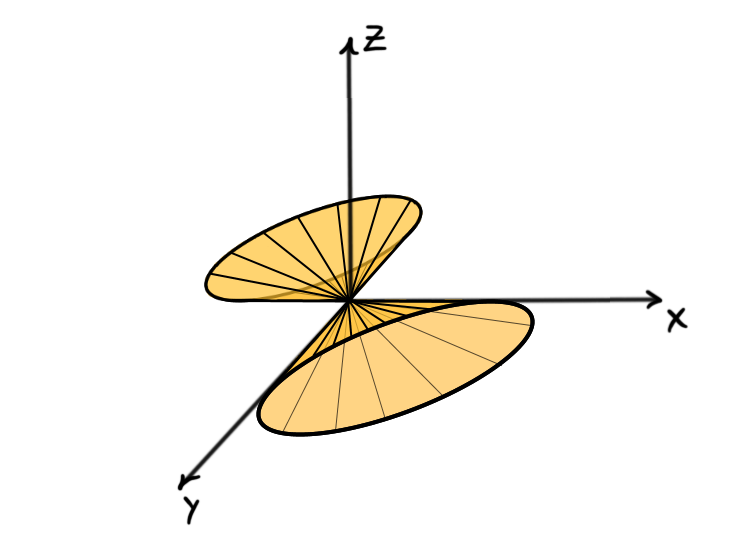
\includegraphics[width=12cm]{img/lecture_7/double_cone.png}    
\end{center}

We denote $\overline{C}$ its image in $\P^2(\R)$. It intersects the plane $z=1$ at the graph of $xy=1$. 

\begin{center}
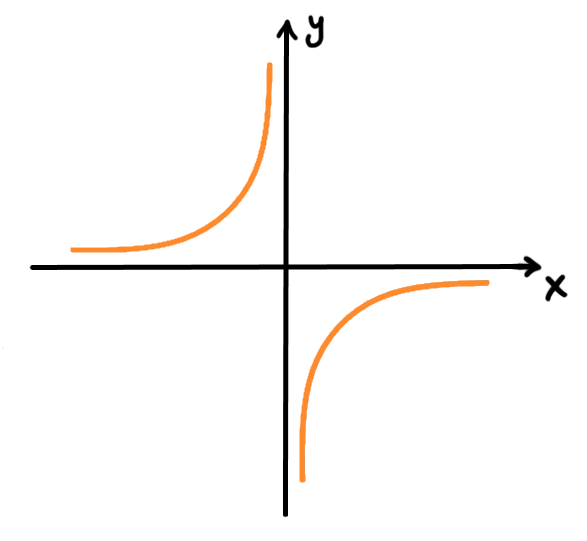
\includegraphics[width=8cm]{img/lecture_7/double_cone_2.png}    
\end{center}

$\overline{C}$ also intersects $V(Z)$ at two points in the $z=0$ plane, namely $[1:0:0]$ and $[0:1:0]$, i.e. the two axes. 


We see that the two ``points at infinity'' correspond to the asymptotes of the graph that intersects $z=1$, i.e. the asymptotes of $xy=1$. 

\begin{problem}
Where does $\overline{C}$ intersect the projective line $x-z=0$?

\begin{solution}

\end{solution}
\end{problem}
\todo[inline]{Solution}

We see by the previous problem that the conics (circles, ellipses, hyperbola, parabola) are all ``affine constructs''. In projective space, these properties could be characterized by how the conic cuts the line at infinity. It can cut it into $0$, $1$ or $2$ parts, which correspond to the three types of conics. 